% \newpage
\section{Mitigating Attacks}
\label{sec:security}
Having introduced the design of the system, we now turn our focus to one of our key goals: protecting the privacy and value of system participants.
% In this section, we discuss potential attacks that can be made against our solution. 
% Attacks may come from multiple directions-- advertisers trying to gain access to users without paying, malicious attackers trying to undermine the privacy of users, or users trying to unfairly obtain money from advertisers.
% We first note that because our solution requires third party entities to pay in order to access the user, any entity who obtains location
% information must pay in order to monetize that information. Having said that, there can be inference
% based attacks, where blacklisted locations of users can be learned by comparing against other users' information
% or ad-networks can learn more about a user, given that mobility patterns are periodic. We deal with such attacks next.

\subsection{Attacks on the Value of User Data}
% There are a variety of ways ad-networks may try to take advantage of information from the system without properly compensating the user. 
% Our system prevents that such adversary economically benefits from doing so.
% Our system prevents an adversary economically benefiting by doing so.
Our system prevents an adversary from economically benefiting by using information about a user without properly compensating her.

Ad-networks may try to build up interest profiles of users over time in order to better target ads later \emph{without} compensating the user. Even if a user's anonymous ID is changed regularly, human mobility patterns are periodic and somewhat predictable, making it easy to link a current anonymous ID to an older one\footnote{Note this profiling works on \emph{non}-blacklisted locations only.}. Our system does not prevent such profiling, and it even makes it easier as the market announces which data is for sale. However, we ensure that this strategy has no economic benefit, for the following reason: all traffic flows go through a proxy, and an ad network who does not pay will receive the identity and location of a user, but a random temporary ID. Then the ad-network, although it has a rich profile of user $u$, is not able to recognize $u$ as the recipient of an ad. For the same reason, ad-networks do not gain by colluding or reselling the information. Unless a payment is made, the identity and location of $u$ is unknown, and the profile alone does not aid targeting. % suffice to target.

% In any case, an ad-network can only obtain location data if that location does \emph{not} appear on a user's blacklist.
% Thus, any data used to build an interest profile will be data the user is comfortable releasing.
% Because a user's anonymous ID is changed regularly, it takes extra effort on the part of the advertiser to 
% MORE?

A related issue is trajectory-based profiling. If an ad-network learns the habits of a particular user over time, the ad-network can show ads based on where a user \emph{is likely to be} rather than paying for an exact location. Again, ad-networks must always pay to be able to access a user's identity. 
 % only knows that a user visits a location if the user has not blacklisted it.
Care must be taken, however, to make sure that a user does not unwittingly display information about a visited blacklisted location based on her trajectory: \eg~ location B is sensitive and locations A and C are not, and the only way to get to C from A is via B). If Alice checks in at point A and then at point C, ad-networks may infer that she visited B. Such attacks are not likely, and can be dealt with by ensuring that after visiting a blacklisted location a minimum amount of time has passed before disclosing a location. 

One concern is if an app works to circumvent the proxies and leak information about either the location or the identity of the user. 
% Against location leakage, one solution is to not reveal the location to the application if that is doable, and if the OS properly implements a user's privacy preferences. 
Against location leakage, one solution is to substitute a fake location to the app if it does not disrupt service~\cite{Hornyack:2011wq}.
An adversarial app could monitor the location market and try to associate an anonymous user profile with a particular device. Combined with a profiling attack, it can then send targeted advertisements without compensation by recognizing this device from now on. This is a costly attack and can be prevented if OSes separate their advertising services from applications~\cite{Leontiadis:2012} or if the users does not need a permanent ID for this application. Note also that, since UIDs are changed periodically, the profile cannot be updated without paying and hence loses some value over time.
% a user over time, and try to associate a user's anonymous data with a certain device, thus gaining the 

\subsection{Attacks on User Privacy}
\label{sec:inference}

We study the robustness of our solution against a form of attack based on \emph{inference}.
We consider a malicious adversary whose goal is to predict the visits to blacklisted locations of 
a specific user with some accuracy.
This may seem a priori impossible since whenever a user visits a blacklisted location, no information about this visit 
is sent or shared anywhere. 

However, because mobility patterns tend to be periodic and similar people may have similar mobility patterns, an adversary 
may be able to discover something about a specific user's blacklist by comparing their publicly available location information 
with the full (including blacklisted) location information of `compromised users'.
This auxiliary location information could be obtained via hacking or a malicious or buggy application.
% However, one could argue that even if an adversary cannot start from information exchanged in transactional location privacy to make this inference, this adversary might be able in some cases to first gather some partial auxiliary information about some nodes and to \emph{augment} this information using our scheme. 
Inspired by de-anonymization techniques based on auxiliary information~\cite{Narayanan:2008iu}, we now pose the following question:~``Can an adversary with the full knowledge of the location information of a significant 
fraction of users predict the blacklisted locations of other users with high accuracy?'' 
We test this on a large dataset of Foursquare checkins.
Intuitively, the sparsity of locations and checkins in this dataset allows for strong attacks of this kind.

\newcommand{\simil}{\textrm{Sim}}
\newcommand{\spann}{\textrm{span}}
As in the de-anonymization technique, we consider a similarity score $\simil(u,v)$ between two users based on common visits. Let $L_u$ denotes the places that are visited at least $1$ time by $u$. We define similarity as:
\[
\simil(u,v) = \sum_{l\in\setL} \frac{1}{\spann(l)} \mathbb{I}_{l\in L_u\cap L_v} \vf
\textrm{for}\; 
\spann(l) = \sum_{u\in\setU} \mathbb{I}_{\{l\in L_u\}}\ff
\]
Note that by doing so we weight more the co-occurrence of a rare location as a sign of similarity between two nodes.

The attack then proceeds as follows. For a given keyword $k$, the attacker looks at all accounts that visited a location tagged with $k$. For simplicity we will say that such a user visits keyword $k$. These are the probes used to find similar users who are more likely to behave like them. For a given user $u$, the adversary first locates the $n=10$ closest users that are compromised in terms of similarity $v_1,\cdots,v_{n}$. 
The attacker then computes the following weighted sum:
\[
P(u) = 
\frac{1}{\sum_{i=1}^{n} \simil(u,v_i)} 
\sum_{i=1}^{n} \simil(u,v_i) \mathbb{I}_{\{v \midwor{\footnotesize visits keyword}k\}}.
\]
It then predicts that $u$ visits locations associated with keyword $k$ if and only if $P(u)\geq \theta$ where $\theta\in[0;1]$ is a parameter that allows a trade off between accuracy and aggressiveness of the reconstruction technique.

We empirically study the effectiveness of this attack using 1.3 million checkins at 460,663 locations from 40,578 Foursquare users, obtained through crawling publicly available tweets of checkins between March and August 2011. Each Foursquare location is marked with a category, which we assigned to be that location's keyword. In this attack, we consider a severe case where the adversary has compromised 20\% of all accounts. We vary the value of $\theta$ from 0 to 1 and plot the precision-recall of this attack for various keywords in Fig.~\ref{fig:inference}.
\begin{figure}[tbp]
\centering
\begin{tabular}[1]{cc}
\hspace{-0.35cm}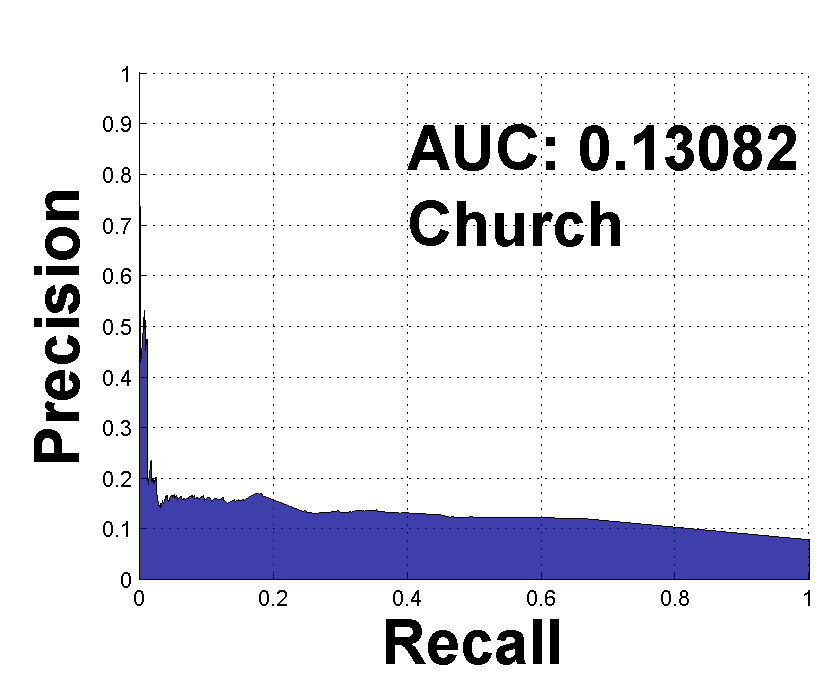
\includegraphics[width=1.5in]{fig/keyword/inf_church_pr.eps}
&
\hspace{-0.35cm}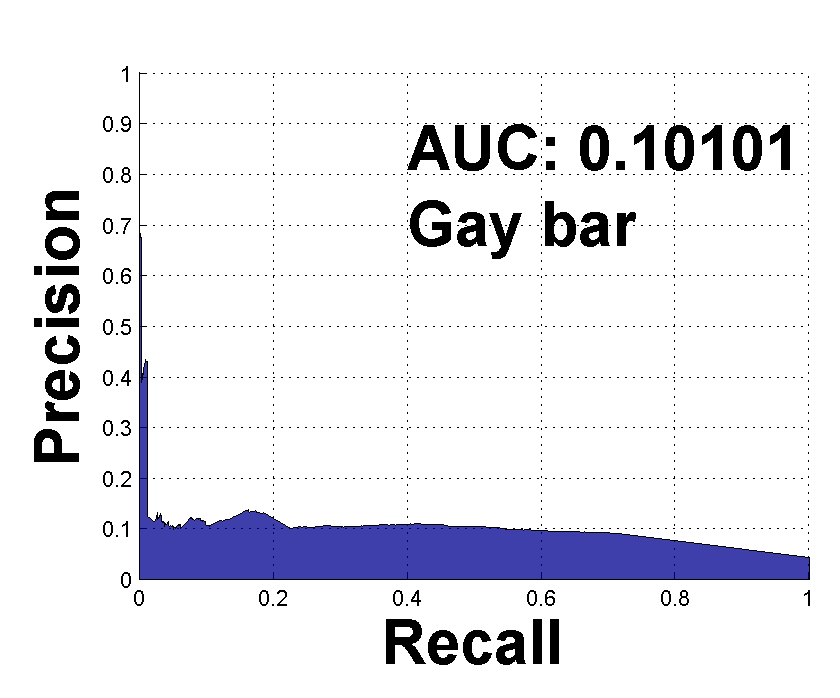
\includegraphics[width=1.5in]{fig/keyword/inf_gaybar_pr.eps}
\\
(a) & (b) \\

\hspace{-0.35cm}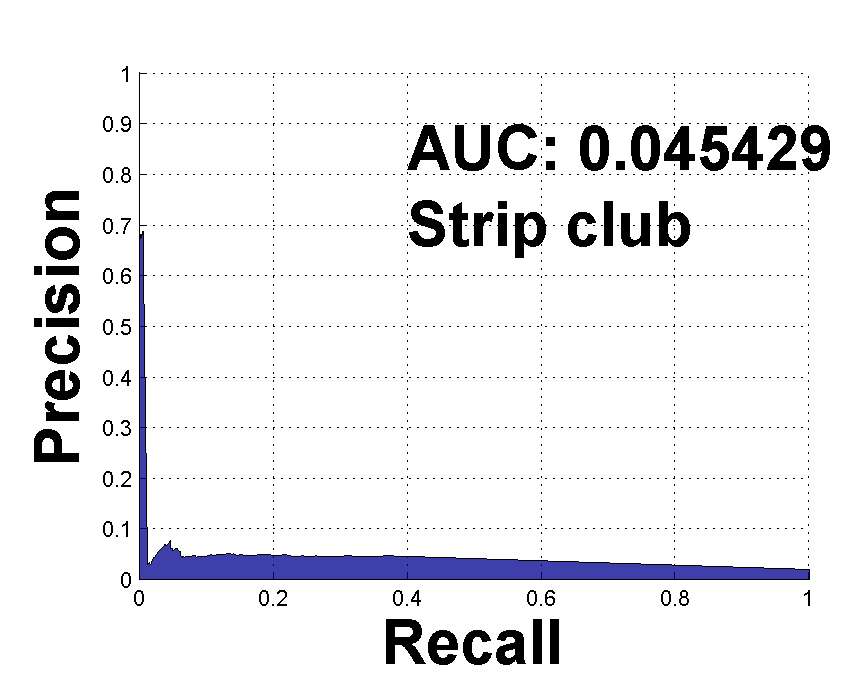
\includegraphics[width=1.5in]{fig/keyword/inf_stripclub_pr.eps}
&
\hspace{-0.35cm}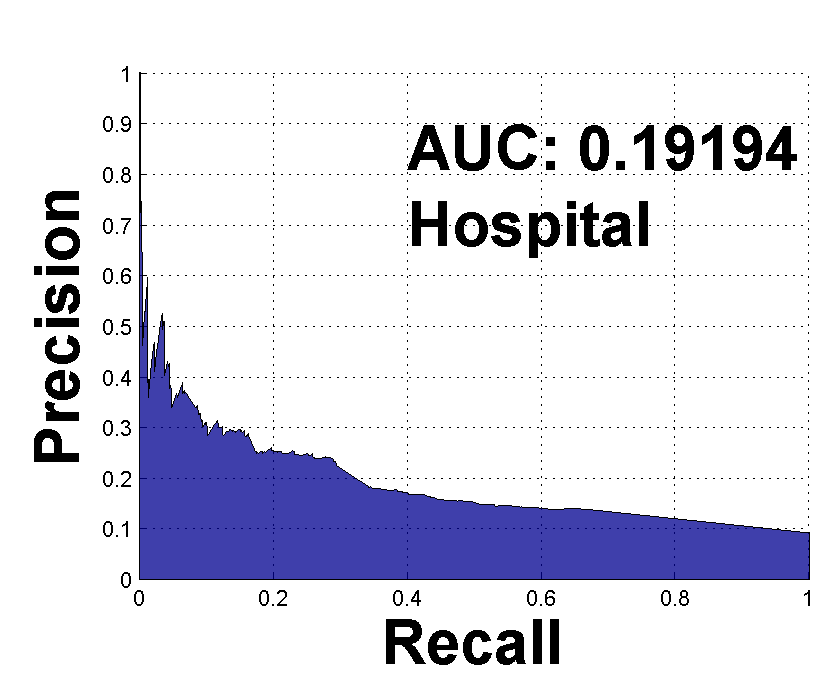
\includegraphics[width=1.5in]{fig/keyword/inf_hospital_pr.eps}
\\
(c) & (d) \\
\end{tabular}
\caption{Precision-Recall curves for four sensitive keywords: (a) Church (b) Gay Bar (c) Strip Club (d) Hospital}
\label{fig:inference}
\end{figure}
As one can see, this attack is rarely effective, even in such extreme case where many user accounts have been compromised. The area under the curve is almost always very small. 
This turns out to be true even for locations that are sparse, as it is much more difficult to guess right when only a handful of users are visiting a rare location. 

This points to an interesting difference between inference in our scheme and de-anonymization attacks. While de-ano\-ny\-mi\-za\-tion attacks always benefit from sparsity since the data are present in a sanitized form, in our context, the attack does not always benefit from sparsity. This is because a minimum critical mass of typical behavior is needed in order to run inference. This shows that a proper choice of blacklist could potentially protect many locations, even as several accounts are compromised in the system. 

% Not sure where Bala wanted me to put this...

% More work remains to be done in this area. 
% One promising direction of study would be the effect of translating locations to keywords on k-anonymity in large traces.
% Another topic to be considered is trade-offs between time granularity and privacy.

\subsection{Attacks on Advertiser Revenue}
We now consider if advertisers can unfairly lose money to unscrupulous users of the system.
Because users are paid when they are accessed by advertisers, they have an incentive to view or click on many ads, even when they are not interested in the displayed products, to artificially boost their profile's value to derive more money from each click.
We label these activities ``user fraud." %different name??

% It is important to note that digital user fraud is really a special case of invalid traffic in online advertising.
User fraud is a special case of invalid traffic in online advertising.
According to Google's Ad Traffic Quality Resource Center, ``invalid traffic includes both clicks and impressions ... [that are] not the result of genuine user interest. This covers intentionally fraudulent traffic as well as accidental clicks and other mechanically generated traffic."\footnote{\url{www.google.com/ads/adtrafficquality/index.html}}
% This definition applies equally well to any clicks or impressions a user creates in order to game the system.
A request for an ad within our system is just like a request for an ad in the current ad ecosystem, but with some privacy-protecting filtering and potential additional location information.
Thus, previous techniques used to identify invalid traffic can be used to identify user fraud.
% Recently, there has been a variety of research on this subject.
There is a lot of recent research on this topic.
Dave et al propose methods to fingerprint click spam~\cite{clickspam}.
Haddadi uses ``bluff ads", ads designed to not appeal to humans and thus only be clicked by bots, to defeat click fraud~\cite{bluffad}.
Information on the structure of Google's click fraud detection system is available ~\cite{googleClick1}. %, ~\cite{laneGiftReport}.
Beyond academia, multiple startups exist that estimate the rates of click fraud,
such as Adometry, Visual IQ, and ClearSaleing~(%\footnote{
\url{www.adometry.com}, \url{www.visualiq.com}, \url{www.clearsaleing.com}
%}
).
% We first note that such a problem is only as difficult as that of standard click fraud on the web.
% The amount of money to show one impression of an ad on the internet is exceedingly low, meaning the amount of money a user can expect to get from viewing an impression in our system will also be low.
% Thus, we only need to worry about 

Additionally, it is easier to detect user fraud than traditional invalid traffic because location information is more constrained than web-browsing.
Users are physically constrained in how far they can travel in a certain period of time
and typically display periodic mobility patterns, returning to their homes at night and spending week days at work locations.
A more extreme use of physical constraints would be to use location tags; fingerprints extracted from ambient signals at a specific location at a specific time~\cite{NarayananTLHB11}.
These constraints can be used to filter out automated attacks on a system. 
For example, if a user appears to be traveling faster than is physically possible, we can remove them from the system or verify their accounts with a Captcha or phone call.
Because of these physical constraints, and because click fraud prevention techniques can easily be applied to our system, we believe that our system is no more vulnerable to gaming than current online advertising. 
% Although click fraud is considered an open problem by the research community, 
The ongoing viability of online advertising shows that our solution should likewise not be derailed by invalid traffic.

% Beyond digitally generated location fraud, 
Beyond automated attacks, users might ``physically" attack the system by simply going to a high value location in order to appear more valuable to an advertiser than they actually are.
Again, techniques to combat click fraud can be employed here.
Click fraud techniques must deal with situations in which users actually click links to unfairly gain money, a nice analogy to this form of attack.
Beyond this, traveling to a location takes significant time and effort and will likely be too costly to be a viable way of making money.

% Traveling to a location takes significant time and effort. Such time and effort has an opportunity cost. 
% In order to make such an attack worthwhile, the user would have to have a very valuable profile. We don't anticipate profiles having such a high value unless the user has made multiple purchases in the past, in which case the advertiser would be compensated appropriately.
% Finally, the market should help deal with these attacks. We believe that valuable profiles will be distinguishable from worthless ones. The market should then be able to appropriately price them. To aide in this distinction, some reputation scheme could be added on top of the user's profile. For example, a user could receive a rating based on how often they respond to advertising.

% Gaming of the system is certainly an issue and an area for future study. 
% However, we believe that such concerns are no more difficult than the current click fraud situation facing online advertising.
% Given that online advertising is a thriving field in spite of these concerns, we feel that gaming does not pose a disastrous risk to our system.
